% Transformer pipeline with SAE-gate and linear projector positions
\documentclass[tikz,border=5pt]{standalone}
\usepackage{xcolor}
\usepackage{fontspec}
\usetikzlibrary{arrows.meta,shapes.geometric,fit,calc,shadows.blur}

% Define color scheme
\definecolor{primaryblue}{RGB}{41,128,185}
\definecolor{secondarygreen}{RGB}{39,174,96}
\definecolor{accentorange}{RGB}{230,126,34}
\definecolor{warningred}{RGB}{231,76,60}
\definecolor{lightgray}{RGB}{236,240,241}
\definecolor{darkgray}{RGB}{52,73,94}

\begin{document}
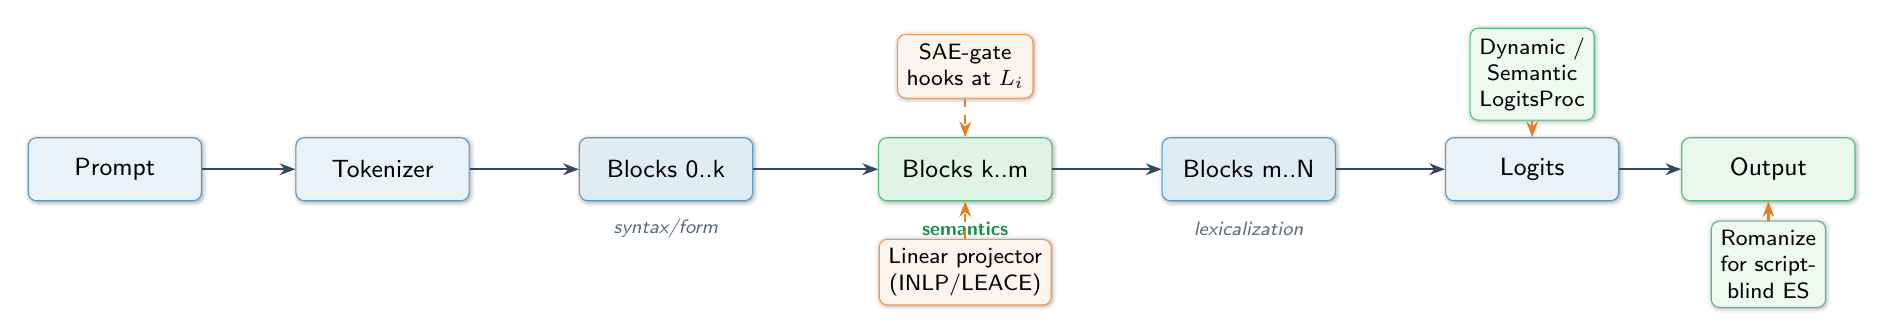
\begin{tikzpicture}[
  node distance=8mm and 14mm,
  block/.style={
    draw=primaryblue!80,
    fill=primaryblue!10,
    rounded corners=3pt,
    minimum width=22mm,
    minimum height=8mm,
    align=center,
    font=\sffamily\small,
    blur shadow={shadow blur steps=5, shadow xshift=0.5pt, shadow yshift=-0.5pt}
  },
  small/.style={
    draw=secondarygreen!80,
    fill=secondarygreen!8,
    rounded corners=3pt,
    minimum width=14mm,
    minimum height=7mm,
    align=center,
    font=\sffamily\footnotesize,
    blur shadow={shadow blur steps=3, shadow xshift=0.3pt, shadow yshift=-0.3pt}
  },
  intervention/.style={
    draw=accentorange!80,
    fill=accentorange!8,
    rounded corners=3pt,
    minimum width=14mm,
    minimum height=7mm,
    align=center,
    font=\sffamily\footnotesize,
    blur shadow={shadow blur steps=3, shadow xshift=0.3pt, shadow yshift=-0.3pt}
  },
  line/.style={-{Stealth[length=2mm]}, thick, draw=darkgray},
  dashedline/.style={-{Stealth[length=2mm]}, thick, draw=accentorange, dashed},
  annot/.style={font=\sffamily\scriptsize, align=center, text=darkgray!80}
]

% Input and tokenizer
\node[block] (inp) at (0,0) {Prompt};
\node[block] (tok) at (3.4,0) {Tokenizer};
\draw[line] (inp) -- (tok);

% Early blocks (syntax/form)
\node[block, fill=primaryblue!15] (b0) at (7.0,0) {Blocks 0..k};
\node[annot] at ($(b0.south)+(0,-3.5mm)$) {\textit{syntax/form}};
\draw[line] (tok) -- (b0);

% Mid blocks with interventions - highlighted
\node[block, fill=secondarygreen!15, draw=secondarygreen!80] (b1) at (10.8,0) {Blocks k..m};
\node[annot, text=secondarygreen!80!black] at ($(b1.south)+(0,-3.5mm)$) {\textbf{\textit{semantics}}};
\draw[line] (b0) -- (b1);

% SAE-gate hook
\node[intervention] (sae) at ($(b1.north)+(0,9mm)$) {SAE-gate\\hooks at $L_i$};
\draw[dashedline] (sae) -- (b1);

% Linear projector hook
\node[intervention] (proj) at ($(b1.south)+(0,-9mm)$) {Linear projector\\(INLP/LEACE)};
\draw[dashedline] (proj) -- (b1);

% Late blocks
\node[block, fill=primaryblue!15] (b2) at (14.4,0) {Blocks m..N};
\node[annot] at ($(b2.south)+(0,-3.5mm)$) {\textit{lexicalization}};
\draw[line] (b1) -- (b2);

% Logits/processor
\node[block] (logits) at (18.0,0) {Logits};
\draw[line] (b2) -- (logits);
\node[small] (proc) at ($(logits.north)+(0,8mm)$) {Dynamic /\\Semantic\\LogitsProc};
\draw[dashedline] (proc) -- (logits);

% Output and romanization
\node[block, fill=secondarygreen!10, draw=secondarygreen!80] (out) at (21.0,0) {Output};
\draw[line] (logits) -- (out);
\node[small] (rom) at ($(out.south)+(0,-8mm)$) {Romanize\\for script-\\blind ES};
\draw[dashedline] (rom) -- (out);

\end{tikzpicture}
\end{document}
